\documentclass[a4paper,11pt]{article}
\usepackage{dmasproject}
% if you need additional LaTeX packages, add them here
\usepackage{graphicx}
\usepackage[export]{adjustbox}
\usepackage{subcaption}
\graphicspath{ {./Design of Multi Agent Systems/} }

\title{Modeling civil violence in a rebellion}
% sort your names alphabetically by last name
\author{
  Sam Reswinraj Abraham (s4248325)
  \\
  Amit Bharti (s4417526)
  \\
  Niels Burgler (s3665828)
  \\
  Abhishek Ramanathapura Satyanarayana (s4304675)
}
\date{Beta version, October 2021} % change this accordingly

\begin{document}
\maketitle

\begin{abstract}
\textbf{Civil violence is becoming a common phenomenon, resulting from high level of inequality and corruption, with digital media acting as a catalyst in recent times. Although a lot of study has gone into this area, the influence of corruption, spread and bias of information through digital media, and centralized and strategic movement of a rebellion are yet to be taken into account. Our model focuses on carrying forward the results of Epstein's \cite{epstein2002modeling} study in order to examine the consequences of cops defecting and the influence of social media in a multi-agent setting. It was found that a centralized rebellion, as a result of social media, is harder to silence.}  
\end{abstract}

\section{Introduction}
Inequality is growing for more than 60 percent of the global population leading to rapid rise in corruption, crime rates, and social conflicts. One way of overcoming these challenges is through proper governance. But the advancement in digitization has lead to drastic increase in the amount of people being involved in civil violence around the world, since local issues are being heard by a bigger audience. The importance of understanding and if possible predicting and eventually controlling the trends in the number, variety and intensity of these phenomena cannot be overemphasized.

\subsection{Problem}
Civil violence is a dynamic complex behaviour in which size, intensity, grievances, greed and loss of life/property play a major role in deciding the outcome of the situation. Examining civil violence can only really be done in hindsight, by examining past riots or rebellions. By making a model of civil violence, the factors that influence the outcome of a riot or rebellion can be examined quickly and in an ethical way. A lot of work has been done in this are already, but examination of the influence of current technologies is lacking, and the possibility of authorities joining the rebellion is often not taken into account.

\subsection{State of the art}
Epstein's model \cite{epstein2002modeling} is the most prominent model for the study of civil violence because of its simplicity in the attributes and rules used for modeling the agents to explain complex dynamic behaviour. The model uses decentralized cops against decentralized civilians as reactive agents. The model uses two types of agents,  rebels and cops, that exist in a two dimensional grid. The rebels can be active or quiet. The rebels can turn active based on attributes such as the legitimacy of the government and the amount of cops nearby. The cops can arrest active rebels to try and stop the rebellion. More details about Epstein's model can be seen in section 2.1.1, or in \cite{epstein2002modeling}. %Through Epstein's model, it could be inferred that legitimacy is one of the key attributes in outcomes of rebellion dynamics. The sudden decrease in perceived legitimacy could lead to exponential increase in the rebellious activities. The other key attributes that affect the outcome of the rebellion dynamics are cops' position, density and strength.
 
\subsection{New idea}

In our model, we have extended Epstein's model to include the current scenario where people are more connected digitally. We have worked on movement of rebels based on information perceived through digital media. We have also explored cops' defection and looked out for the new equilibrium that would develop. Our multi agent model aims at running complex dynamics of rebellion situation in a controlled environment considering realistic attributes based on cops' bias and digital media involvement, in order to predict the future outcomes based on various factors.

\section{Method}

\subsection{Simulation model}
Our model is an extension of Epstein's model \cite{epstein2002modeling}. To explain how our model works, we will first give an explanation of Epstein's model, before explaining the additions and modifications we made.
\subsubsection{Basic Model}
First, our model has two distinct types of agents: the cops and the rebels. The rebels are not always actively rebelling. Instead, this depends on the level of their grievance, the the risk of actively rebelling, and their risk aversion. These values are all calculated in the same way as in Epstein's model \cite{epstein2002modeling}. For the grievance, the following formula is used:
\[ G = H(1-L) \]
where G is the grievance, H is the hardship, and L is the legitimacy. Hardship represents the personal hardship of a rebel and is thus heterogeneous. Its value is drawn separately for each rebel from a uniform distribution from 0 to 1. The legitimacy is a value between 0 and 1 that represents the perceived legitimacy of the government. %The exact value can be set by the user of the model. The value of L is the same for every rebel.\\
%The risk of actively rebelling is different for every rebel. It is dependent on the amount of cops that the rebel can see, and the amount of active rebels the rebel can see. The rebel counts themselves for the latter of these, even if they are not active currently. This is because the rebel wants to know how likely they are to be caught if they started actively rebelling.%
The exact formula for the arrest probability is:
\[ P = 1 - exp[-k(C/A)_v] \]
where P is the probability of arrest, C is the amount of cops that the rebel can see, A is the amount of active rebels that the rebel can see, and k is a constant that ensures a proper value of P when C = 1 and A = 1.
Using the arrest probability and the risk aversion of a rebel, the net risk can be calculated using the following formula: $N = RP$; where N is the net risk, R is the rebels' risk aversion, and P is the rebel's arrest probability.\\
Based on the net risk and the grievance, a rebel decides whether it becomes active or quiet. This is done using the following rule:
\[\text{Rebel Rule: If } G - N > T \text{ become active, otherwise remain quiet}\]
where T is a predetermined threshold.\\
Following Epstein's model \cite{epstein2002modeling}, the cops do not suffer from any hardships or grievances. Instead they follow only one rule:
\[\text{Cop Rule: Arrest a random active rebel within vision}\]
When a rebel is arrested, they are jailed for an amount of ticks drawn from a uniform distribution between 0 and $J_{max}$, the maximum jail time. While a rebel is jailed, they no longer perform the rebel rule, and their patch is considered unoccupied. When a cop arrests a rebel, the cop moves to the rebels' patch.
%Epstein does not specify what arresting the rebels means exactly, only that an arrested rebel goes to jail for an amount of time drawn from a uniform distribution from 0 to $J_{max}$ (the maximum jail time), that the patch they were/are on is considered unoccupied while they are in jail, and that they leave jail exactly as aggrieved as when they entered. For our model, we can be more exact about what arresting a rebel does. When a cop arrests a rebel, the cop moves to that rebels spot and renders the rebel jailed for $U(0,J_{max}$) ticks. This means that the rebel is turned quiet, and no longer uses the rebel rule until they get out of jail. The rebel's patch is no longer deemed occupied, which means that other agents can occupy it instead.
\\
In addition to these rules that are specific to the rebels and cops, there is also a rule that both of them use: the movement rule. Here - An agent always uses the movement rule before using the rebel or cop rule. This rule can be described in the following way:
\[\text{Movement Rule: Move to a random empty patch within your vision}\]
\subsubsection{Modified model formulation for cop defection}
The modeling of cops is crude in the Epstein's model. The model does not include scenarios where cops defect and support the rebellion's cause. In Epstein's model, it is assumed that all cops are loyal to the authority, which is ideal. However, in the real world, this is not the case. There may be various factors which may drive a cop to defect and support the rebellion. In our model, we consider a few realistic attributes which may play a role in cop defection in the real world \cite{policeintegrity, policecorruption}.

In our model, we consider a small percentage of total cops to be plausible cop candidates for defection and rest of the cops to be normal cop candidates. The number of plausible cop candidates for defection that actually defect depends on a simple set of rules which is similar to that of the behaviour of rebels in Epstein's model\cite{epstein2002modeling}.
The following assumptions are made in our cop defection model:
\begin{itemize}
    \item All the cops have the same rank, 
    \item The defected cops do not reveal to the other cops that they have defected (however, the rebels know which cops have defected and actually support the rebellion cause), and
    \item There will be only 2 states for a cop, either defected or not defected
\end{itemize}
In our model, the rule remains the same for non-defected cops. The following is the rule for defected cops:
\[\text{Defected Cop Rule: The defected cops will not arrest any active rebels in their vision}\]

Currently, our model considers the following attributes for the behaviour of cop defection: personal bias against the authority, monetary benefits received for the service, greed, personal hardship and perceived legitimacy of the authority (different from that of rebels since cops represent a different set of population in the society) \cite{epstein2002modeling, policeintegrity, policecorruption, policeattitude}.

The tendency to defect due to grievance, $T_{grievance}$, is computed using
\[T_{grievance} = H (1 - L)\]
where $H$ is the hardship faced, $L$ is the perceived legitimacy of the authority.

The tendency to defect due to greed, $T_{greed}$, is computed using
\[T_{greed} = (1 - \lambda) G\]
where $\lambda$ is the benefits received for service and $G$ is the greed.

The average tendency to defect , $T_{avg}$, is simply the average of the two tendencies.
\[T_{avg} = \frac{T_{grievance} + T_{greed}}{2}\]

The probability to defect , $P_{def}$, is computed using the following formula
\[P_{def} = 1 - exp(-\frac{zB}{1 - T_{avg}})\]
where $B$ is personal bias against the authority, $T_{avg}$ is the average tendency to defect and $z$ is a constant. We set $z=1.8$ which was found by continuous simulation.

The following is the rule for cop to transition to defect state
\[\text{Rule for transition of cop state to defect: if $P_{def} > Threshold_{def}$}\]
We use $Threshold_{def} = 0.7$, which was found by continuous simulation.

In our model, we have assumed that defected cops do not arrest the active rebels in their vision. This changes the formula to compute probability of arrest of active agents slightly, $P_{updated}$. The following is the updated formula
\[ P_{updated} = 1 - exp[-k(\frac{C_{nd}}{A})_v] \]
where $C_{nd}$ is the count of cops, in the rebel's vision, who have not defected. The further sections capture some significant observations in the overall dynamics of rebellion due to the introduction of our cop defection model as an addition to Epstein's model\cite{epstein2002modeling}.

In our current formulation for cop defection, the state transition of plausible cop candidates does not take into account any dynamic attributes which change during the simulation of the rebellion dynamics. This is a drawback of the current formulation of cop defection model. Our future work will include an effective formulation for the behaviour of cop defection to take into account some dynamic attributes.
\\

\subsubsection{Modified model formulation for Social Media}
When we think about social media, connectivity is the first thing that comes to our mind. So we have made two additions/modifications to Epstein's model. First, we explored connectivity with respect to movement of agents. That is, we changed the movement of the rebels from random in Epstein's model to three different types of movement: Avoidance, Custom and Random movement for the rebels. Similarly cops were assigned Random and Custom movement.
\\
The Avoidance movement is based on the idea that the access to social media enables the rebels to spread information about the locations of the cops. Because of this, the rebels are now able to avoid the cops. Every patch stores its distance to the closest cop. The new movement rule for the rebels becomes the following:
\[\text{Rebel Movement Rule: Move to a random empty patch within your vision with } D_{new} <= D_{current}\]
where $D_{new}$ is the distance from the new patch to the closest cop, while $D_{current}$ is the distance from the patch the rebel is currently standing on to the closest cop. 
\\
The custom rebel movement takes several factors into account. First, specific areas are added to the map which may act as a hot-spot due to its location or financial gain (robbery from retail store) \cite{davies2013mathematical}. Location of crime is closely related to criminal awareness space i.e. location of opportunities and offenders knowledge \cite{brantingham1993nodes}. Therefore we have small patches of different areas in the model and they have different values assigned to them to indicate how desirable it is for a rebel to move there. Different types of area in the model are retail shops, government buildings, police stations, and parks and their predetermined amounts are randomly placed on the map, each with predetermined values depends on potential reward at different sites. Six retail shops are placed with a value of 4, three government buildings are placed with a value of 10, two police stations are placed with a value of -10, and two parks are placed with a value of 6. The retail shops, government buildings, and police stations each occupy a 3x3 space on the map, while the parks occupy a 5x5 space.
\\
The second variable of the custom rebel movement is the distance to the patch. Rebels seeks to minimize cost so they prefer going to a patch that is closer to them.
\\
The third variable of the custom rebel movement is the number of friends near to the patch. Since people tend to act/move together with their known ones and they are more aware of the surrounding at which their friends are so this parameter will benefit the rebels while choosing their next step. In the model setup, rebels are divided into four equal groups, or `teams'. These groups represent people that are in the same online social circle and we are assuming that teams remain same through out the simulation. While calculating the next move, a rebel looks at every unoccupied patch in his vision and counts the amount of rebels that are in the same team in a radius of 2 around that patch. Rebels tend to move to a tile that is close to their friends.
\\
The fourth, and final variable of the custom movement is to avoid patches that are closer to the cops. This is done in the same way as in the avoidance movement. 
\\
Putting together, in custom rebel movement each rebel will look into all these parameters in his vision and select the empty patch that has maximum value of $v_{total}$ according to below equation.

\[v_{total} = a1 * v_{area} - a2 * distance_{patch} + a3 * friends + a4 * distance_{cops}\]
\begin{center}
where a1 + a2 + a3 + a4 = 1.
\end{center}
After parameter tuning we came up with coefficient values of a1, a2, a3 and a4, which are 0.2, 0.2, 0.25, and 0.35, respectively. 
\\
The user of the model can enable and disable terms of this formula as desired. This means that the effects all the different parts, such as the areas, can be examined separately, or all at once. In figures \ref{fig:subimNormal} and \ref{fig:subimCustom} the difference in the view when turning areas and friends off or on can be seen. In \ref{fig:subimCustom}, the different areas are represented using different shades of green and yellow, and the different friend groups are indicated by the numbers 1 to 4 on the blue dots.\\

\begin{figure}[h]
 \begin{subfigure}{0.4\textwidth}
 \centering
  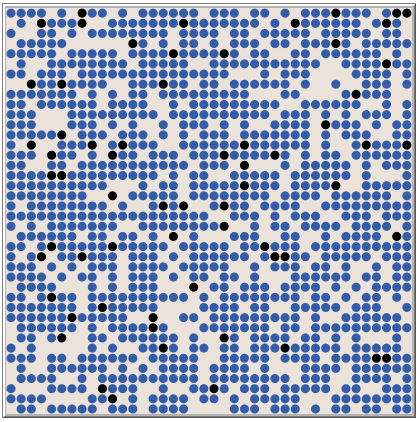
\includegraphics[width=0.8\linewidth, height=6cm]{NormalExample.PNG} 
  \caption{View with areas and friends disabled}
  \label{fig:subimNormal}
 \end{subfigure}
 \begin{subfigure}{0.6\textwidth}
 \centering
  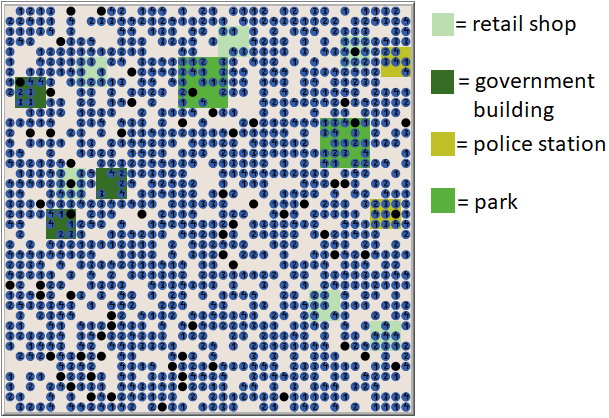
\includegraphics[width=0.9\linewidth, height=6cm]{CustomExample.PNG}
  \caption{View with areas and friends enabled}
  \label{fig:subimCustom}
 \end{subfigure}
 \caption{Examples of the view}
 \label{fig:ViewExample}
\end{figure}


The custom cop movement is simpler than the custom rebel movement. It depends on two variables, the distance to the patch, and the density of active rebels near the patch. The active rebel density is calculated as follows:
\[density_{AR} = AR_n/C_n\]
where $AR_n$ is the amount of active rebels within the cop vision on the new patch, and $C_n$ is the amount of cops within the cop vision on the new patch. The custom cop movement rule can be described in the following way:
\[\text{Custom Cop Movement Rule: Move to an empty patch within vision with the highest } v_{total}\]
where $v_{total}$ is calculated as
\[v_{total} = c1 * density_{AR} - c2 * distance_{patch}\]
\begin{center}
where c1 + c2 = 1
\end{center}
After parameter tuning we came up with coefficient values of c1, and c2, which are 0.6, and 0.4 respectively.
\\
Again, both terms can be turned on or off by the user to examine their separate influences. 
\\
The second addition we made to the model was the addition of perceived legitimacy, $L_{perceived}$. In contrast to the homogeneous legitimacy that set by the user, perceived legitimacy is personal for every rebel and thus heterogeneous. At model setup, every rebel's perceived legitimacy is drawn from a normal distribution with the mean equal to the legitimacy and the standard deviation equal to 0.1. The rebel rule is modified based on this change. Firstly, perceived legitimacy will replace legitimacy value in all calculations. Secondly, a new action is added to the rebel rule. In every turn, a rebel talks to a nearby rebel about their perceived legitimacy and updates his own perceived legitimacy according to below equation:
\[L_{perceivedOwn} = (L_{perceivedOwn} + L_{perceivedOther})/2\]
where the rebel's own perceived legitimacy and the nearby rebel's perceived legitimacy are being averaged. Currently, this is the only thing that influences the perceived legitimacy of a rebel. This means that, after a certain amount of runs, every rebel will have the same perceived legitimacy, which value will be very close to the actual legitimacy value. In short, the addition of perceived legitimacy does not do much as of yet. However, we do have several plans for the further implementation of perceived legitimacy. First, we want to change the updating function of the perceived legitimacy in such a way that its value is incremented or decremented in steps closer to the other rebel instead of taking the average. Second, we want social media to decrease the rebels' perceived legitimacy \cite{Breuer_2016}, but propaganda to increase the rebels' perceived legitimacy.

\subsubsection{Future Mathematical Modelling for Cop Defection \textit{ (under dynamic conditions ) }}
The current modified model for cop defection does not take into account the dynamic state of the system. Parameters are modelled based on one time inputs (static model) at the beginning of the run cycle. To model it further a ground work on the mathematical modelling has been done. \textbf{This means that the rules described in this section (2.1.4) are not used in the current model.}\\
\\
\textbf{Type of Agents considered for modelling} – \textit{utility agents} \cite{WooldridgeMAS}\\
\textbf{Environment specification} – \textit{cops, rebels, rebellion} \cite{epstein2002modeling}\\
\\It is considered all cop agents in this developed system are utility based working on action sets in the \textit{Action space} to bring about a change in the \textit{State space}. We will be considering state transformers derived as:
\[ T = Ac_i * Ac_j \in \text{O : [E1,E2]}\]
E1 and E2 are specified as such: \[AG : E \longleftarrow Ac;\]
Where, AG = agent (Cop, in this case); E = environment specifier; Ac = Action component\\
\textbf{E1} is defined as the state of the environment where cops defect resulting in change or no change in the Rebellion.\\
\textbf{E2} is defined as the state of the environment where cops do not defect resulting in no change in the studied outcome and performance of the existing system \cite{epstein2002modeling}.\\

Now that the states are established we will be considering parameters to define Utility Functions \cite{WooldridgeMAS} – $U_i$ $\&$ $U_j$
Where – 
  \[U_i \implies \text{Defect function}\]
  \[U_j \implies \text{Non-defect function} \]

A payoff matrix is replaced with the |\textit{Likelihood of defect}| based on “Defect probability”. Based on this $P(C_{def})$, an agent decides between utility functions  $U_i$ or $U_j$, which then results in an Action in the Action space $Ac_i$ or $Ac_j$, thus transforming the state between E1 and E2.\\
\textbf{Logical Statement:}\\
Statement -             \[X_{PLB} \longrightarrow P \oplus  (L \lor P.B)\]
Where, \\
	$X_{PLB}$  = state evaluator - Whether a Cop will defect or not\\
	P = E\{W\} – Cops defecting || Not defecting \\
	L = Loyal || Not Loyal\\
	P.B = Personally Biased || Not Personally Biased\\
\textbf{Draft Formulation for Attributes:}\\
\textbf{A. Personal Bias }

\[P.B = \left(\frac{1}{S.W^n}\right)) * C.S + Random float (P_g) \]
Where,\\
S.W $\forall$ \{0,0.1,0.2,…….1\} $\longrightarrow [\text{no.of agents} / \text{no.of active for } t_i \text{ (per tick) }]$ \\
n = $\sum_{i=0}^q \langle \text{agents Jailed per tick (t)} \rangle$\\
$P_g$ = \{0,1\}  \text{Defined: personal Grievance (Hidden value) }\\
$C.S = ((L_s + L_c) * Legitimacy)$\\
\textbf{B. Loyalty } 
\[L \in S \{0,0.1,0.2,……1\}	\]

And, $L_s = 40\% || 0.4 $; $L_c = 30\% || 0.3 $; $L_r = mx + b$ Where: m = \{Benefits, Individual Character, Agenda, Social welfare\}\\
\textbf{C. Benefits } 
\[B =   \frac{X}{1+X} \textit{(Reducer function)} \] \\
\textbf{Modelling Defect Probability $P(C_{def})$: } \\
While modelling this important aspect several considerations are to be made as follows: \\

1. To add practicality the model designed takes into consideration some of the parameters that will lead to a “wavering” COP behavior. COP agent $\longrightarrow$ defect $\longrightarrow$ readjust (based on payoff for $U_i$/ $U_j$) \\ % for that particular cop agent amongst the COP agent system. A defected COP agent is not modelled to remain defective, instead $\longrightarrow$ remain defected until a certain scenario which would then affect the agents own pay-off matrix with agent termination from the system.  \\

2. Model will take into consideration two set of values for COP agents:
Latent variables (perceived from the system), and Hidden variables (not defined explicitly - priori/posteriori possibilities, agent types based on temperaments)\\ %– ones that are perceived indirectly from other dynamically changing values part of the system. B. Hidden values – these are the values/variables that have to be considered but cannot be shown explicitly in the model (temperament types, loyalty, priori possibilities, posteriori possibilities) \\

3. Model is designed with unknown outputs due to the limited priori possibilities for COP defection. For example, what \% $Ac_i$ of \Big[$P(C_{def})$ * Cop density] will result in strong change in output is unknown.\\ %of the system – time frame of rebellion is extended (this is the base reference value that would indicate changes of considerable amount $\delta H$ $\longrightarrow$ changing the rebellion dynamics).\\ %In other words our Probability to defect might result in localized observations amongst the defected COP agents but might not alter the Global Environment (Rebellion) in any way. \\
\textbf{Assumptions before modelling $P(C_{def})$:} 
\begin{itemize}
    \item COP agent behavior will change Dynamically based on how an agent perceives $U_i \lor U_j$ 
    \item Hidden values – Non Defect Cop in vision-radius; Risk of getting caught (termination of agent from model); Temperament type of agents – sanguine, choleric, melancholic, phlegmatic. 
    \item Priori probability is valued less to create credibility to model designed 
\end{itemize}
\textbf{Modelling Basics: }\\
Probability of defect $P(C_{def})$ will be calculated using \textit{Runge-Kutta} fourth order type of integration based on \textit{Eulers method} \cite{KAELBLING199899} – \\
	\[d_{i+1} = \frac{(y_{i+!} - y_i)}{(t_{i+1} - t_i)}\]

and, 	    $\frac{d_y}{d_t}$ is related to  $y_!$ by $D[f(x)]$ \\

Once the relation of local and global attributes to agents Utility functions $(U_i || U_j)$ is established by $D[f(x)]$, error is readjusted based on Bias, Standard deviations, and Prediction mean square error. \cite{MMD} \\
After the Utility functions are defined, we find the probabilities of $U_i$ or $U_j$ to prevail during one system run cycle. In order for Probability of $(U_i)$ to be greater than probability of $(U_j)$ , it will be developed with values from using – Detection theory \cite{ORLEAN1995257}. \\
   \[(\text{i.e)} P(U_i | y) > P(U_j | y), \text{will be mapped based on posteriori possibilities} \] \\
This probability is then infused with Markov model \cite{KAELBLING199899}  - forward algorithm in Hidden Markov model and Baum-welch Algorithms to estimate $P(C_{def})$. \\



\subsection{Implementation details}

Our model was made using Netlogo 6.2.0. No additional tools or libraries were used.
%Here you should describe the implementation of your simulation.
%Please explicitly mention any programming languages, tools or libraries you used.

\subsection{Experiment design}
To examine the influence of the avoidance movement, we ran the experiments in Table \ref{tab:expAvoid}. All of these experiments were ran with the initial rebel density set to 0.70. The cop defection and perceived legitimacy parts were also turned off to make comparison to Epstein's model possible.
\begin{table}[h]
\centering
\begin{tabular}{lccc}
\cline{2-4}
 & Run 1 & Run 2 & Run 3 \\ \hline
Variable name & \multicolumn{1}{l}{} & \multicolumn{1}{l}{} & \multicolumn{1}{l}{} \\
Cop vision & 1.5 & 7 & 10 \\
Rebel vision & 1.5 & 7 & 10 \\
Legitimacy & 0.80 & 0.80 & 0.80 \\
Max. jail term & 30 & 30 & 30 \\
Initial cop density & 0.04 & 0.04 & 0.04
\end{tabular}
\caption{These experiments were done using Random movement, Avoidance movement, and Custom movement for the rebels.}
\label{tab:expAvoid}
\end{table}
%Did you run multiple different versions of your simulation with different parameters?
%Then explain the different setups here and why you chose them.

%You can also mention here what results you are expecting.

\begin{table}[h]
\centering
\begin{tabular}{lccc}
\cline{2-4}
 & Run 1 & Run 2 & Run 3 \\ \hline
Variable name & \multicolumn{1}{l}{} & \multicolumn{1}{l}{} & \multicolumn{1}{l}{} \\
Cop defection & disabled & enabled & enabled \\
\% Defect cop candidates & 0 & 20 & 20 \\
Cop vision & 7 & 7 & 7 \\
Rebel vision & 3 & 3 & 3 \\
Legitimacy (perceived by rebel) & 0.60 & 0.60 & 0.70 \\
Max. jail term & 10 & 10 & 10 \\
Initial cop density & 0.058 & 0.058 & 0.058\\
Initial rebel density & 0.7 & 0.7 & 0.7\\
Cop benefits & 0.3 & 0.3 & 0.3\\
Cop perceived legitimacy & 0.6 & 0.6 & 0.6\\
\end{tabular}
\caption{The influence of cop defection on rebellion experiments were done using avoidance movement for rebels and random movement for cops.}
\label{tab:copDefect}
\end{table}

To examine the influence of cop defection on the overall rebellion dynamics, we ran the experiments in Table \ref{tab:copDefect}. All the runs were done using avoidance movement for rebels and random movement for cops.

\section{Results}
\subsection{Experiment Results}

\subsubsection{Movement Comparison}
The results of the experiments from Table \ref{tab:expAvoid} are as follows:\\
For run 1, the results are best represented in a single plot. This can be seen in Figure \ref{fig:avoidanceRun1}. Here, we ran the model for roughly 750 ticks. For the first 250 ticks, the movement is set to Random. After this, the movement is set to Avoidance for 250 tick and finally to Custom for the last 250 ticks. In the plot, a clear but small effect of the movement can be seen. As soon as the movement is changed from Random to Avoidance to Custom, the amount of active rebels increases, while the amount of jailed rebels decreases.\\
\begin{figure}[h]
    \centering
    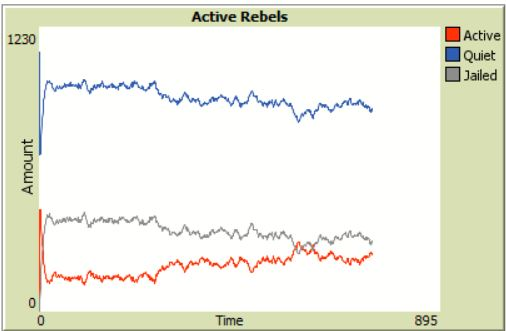
\includegraphics{Run1_Movement.jpg}
    \caption{Run 1 for the Random movement, Avoidance and Custom movement.}
    \label{fig:avoidanceRun1}
\end{figure}
For run 2, we ran all the three models for 250 ticks. The results can be seen in Figure \ref{fig:figRun2}. Here, the Random movement results in rapid spikes of active agents who get captured very quickly. In between these spikes, there is barely any activity. What happens here is that a big group of rebels becomes active simultaneously, which means most of the rebels get captured at about the same time. This means they also get released at roughly the same time, which allows them to become active again very quickly. For the Avoidance and Custom movement, while the spikes are a lot smaller, they are also more frequent. This can be explained by the avoiding movement of the rebels making it harder for the cops to capture them. Instead of capturing almost all the active rebels at once, it takes longer to capture the rebels, which means rebels are already being released from prison before all active rebels are captured. While the rebellion is almost never completely silenced, the rebellion is also never at full strength.\\
\begin{figure}[h]
 \begin{subfigure}{0.33\textwidth}
  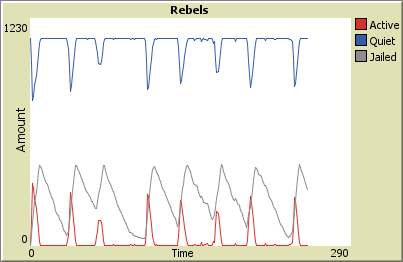
\includegraphics[width=\linewidth, height=6cm]{plotRun2Random.png} 
  \caption{Run 2 with Random movement}
  \label{fig:subimrun2Rand}
 \end{subfigure}
 \begin{subfigure}{0.33\textwidth}
  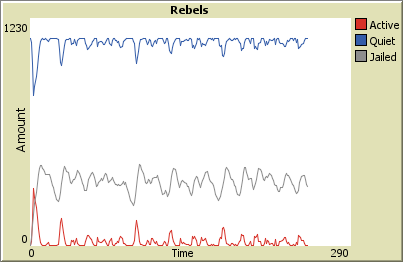
\includegraphics[width=\linewidth, height=6cm]{plotRun2Avoidance.png}
  \caption{Run 2 with Avoidance movement}
  \label{fig:subimrun2Avoid}
 \end{subfigure}
 \begin{subfigure}{0.33\textwidth}
  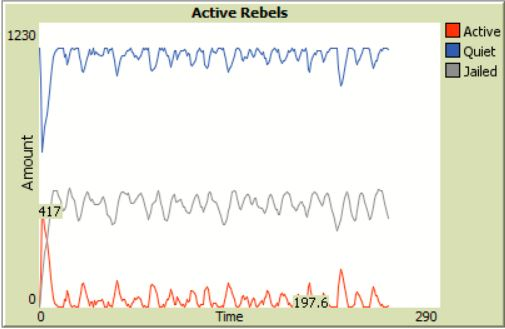
\includegraphics[width=\linewidth, height=6cm]{Run2_Custom.JPG}
  \caption{Run 2 with Custom movement}
  \label{fig:subimrun2Custom}
 \end{subfigure}
\caption{Run 2}
\label{fig:figRun2}
\end{figure}
For run 3, we again ran all the 3 models for 250 ticks. The results can be seen in Figure \ref{fig:figRun3}. This time, for the Random movement the rebels were unable to become active. Apparently, the vision for the rebels results in them seeing too many cops. Because every rebel can see a large amount of cops, not one rebel dares to become active. When using the Avoidance and Custom movement, some rebels are able to move away far enough from the cops to turn active. Because of the high vision value, a lot of other rebels see this and also turn active, leading to a fast peak in active rebels. On the flip-side, the high vision value allows the cop to jail the rebels quite quickly. For the custom movement, the results are very similar to the avoidance movement, except that more rebels are jailed for the custom movement. It seems that the extra terms that the custom movement uses hinder the rebels' ability to avoid the cops.
\begin{figure}[h]
 \begin{subfigure}{0.33\textwidth}
  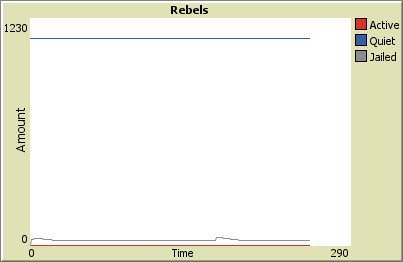
\includegraphics[width=\linewidth, height=6cm]{plotRun3Random.png} 
  \caption{Run 3 with Random movement}
  \label{fig:subimrun3Rand}
 \end{subfigure}
 \begin{subfigure}{0.33\textwidth}
  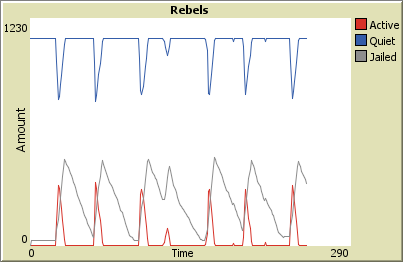
\includegraphics[width=\linewidth, height=6cm]{plotRun3Avoidance.png}
  \caption{Run 3 with Avoidance movement}
  \label{fig:subimrun3Avoid}
 \end{subfigure}
 \begin{subfigure}{0.33\textwidth}
  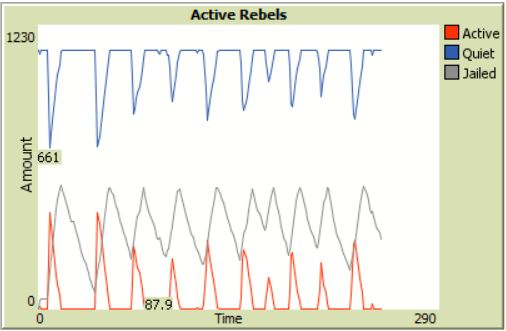
\includegraphics[width=\linewidth, height=6cm]{Run3_Custom.JPG}
  \caption{Run 3 with Custom movement}
  \label{fig:subimrun3Custom}
 \end{subfigure}
\caption{Run 3}
\label{fig:figRun3}
\end{figure}

\subsubsection{Grouping and Local Hot-Spot}
The spatial interaction between rebels shows a tendency of clustering and group formation. As can been seen in figure \ref{Figure : 5}, the rebels are mostly moving in cluster. We can also observe members from same team moving along (highlighted by green circle and zoomed image). In addition local hot-spot areas are acting as key areas for crowd formation (highlighted through dark green circle).
\begin{figure}[h]
    \centering
    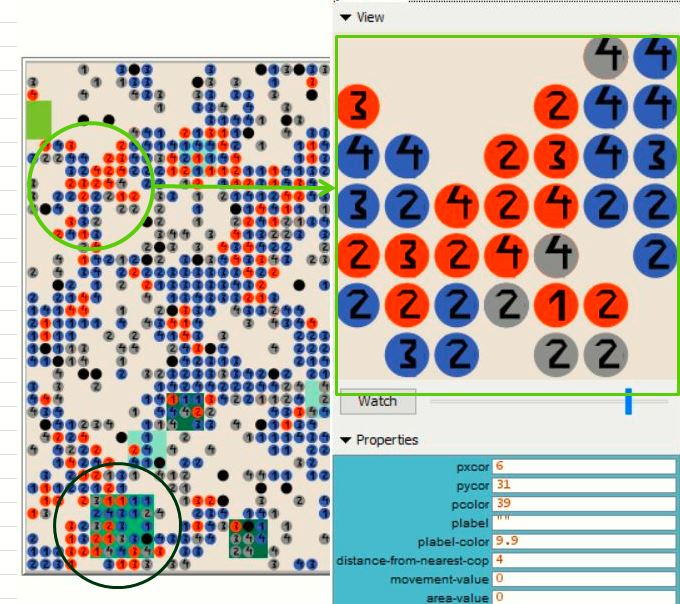
\includegraphics[ height=8cm]{Hot spot and grouping.JPG}
    \caption{Grouping and Local Hot-Spot}
    \label{Figure : 5}
\end{figure}

\subsubsection{Cop defection}
When the cop defection is enabled, there are some cop candidates who have defected (lime color agents in Figure \ref{fig:copDefect3} - run 2 of Table \ref{tab:copDefect}). Figures \ref{fig:copDefect1} and \ref{fig:copDefect2} show the comparison of rebellion dynamics when cop defection is disabled vs enabled. These are for runs 1 and 2 from Table \ref{tab:copDefect}, respectively. We can observe that there is a significant change in the difference between the number of active rebels and quiet rebels when the cop defection is enabled vs disabled. There is a significant increase in the number of active rebels. This is a direct consequence of presence of defected cops, since they do not arrest active rebels in their vision. There was a similar observation for run 3 of Table \ref{tab:copDefect}. For this experiment, the number of active rebels was much higher than that of run 2 of Table \ref{tab:copDefect}.

\begin{figure}[h]
 \begin{subfigure}{0.33\textwidth}
  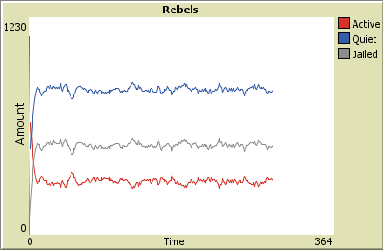
\includegraphics[width=\linewidth, height=6cm]{plot_no_defection_1.png} 
  \caption{No cop defection, table \ref{tab:copDefect} - run 1}
  \label{fig:copDefect1}
 \end{subfigure}
 \begin{subfigure}{0.33\textwidth}
  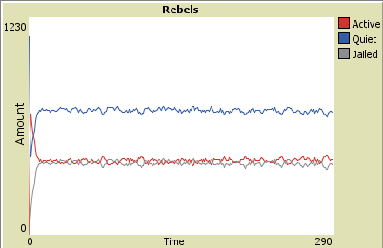
\includegraphics[width=\linewidth, height=6cm]{plot_cop_defection_1.png}
  \caption{Cop defection enabled, table \ref{tab:copDefect} - run 2}
  \label{fig:copDefect2}
 \end{subfigure}
 \begin{subfigure}{0.33\textwidth}
  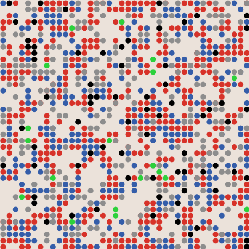
\includegraphics[width=\linewidth, height=6cm]{cop_defection.png}
  \caption{Cop defection enabled, table \ref{tab:copDefect} - run 2}
  \label{fig:copDefect3}
 \end{subfigure}
\caption{Active rebels comparison when cop defection is enabled}
\label{fig:figCopDefection}
\end{figure}

\subsection{General Patterns}
\textbf{Jail time affecting risk factor} - One of the major controlling factors in keeping the rebellion in check was the jail term in Epstein's initial work. We were able to verify its effects. Once the jail term is increased, the number of active rebels reduce and hence the overall rebellion is brought under control.
%Agents i.e. rebels and cops - were given randomized movement and information was allowed to be passed from one rebel agent to the other about “cops in vision” \textit{(News ratio = 1.0)}; there is no observed changes due to the addition of attributes (communication). The model behaves the same as in Epstein's initial model \cite{epstein2002modeling}. Once the jail term is increased, the number of active rebels reduce and hence the overall rebellion is brought under control. %If the jail term is reduced, rebels returning from jail with no effective deterrence and the same value for grievance tend to go active again and be jailed. This cycle continues throughout the run-time of the model. 
\\
\textbf{Individual deceptive behaviour} - 
As observed in Epstein’s model \cite{epstein2002modeling}, we were able to verify the same outputs with our reconstructed model. Agents (rebels and cops) are modeled after simple rules in terms of vision radius. Although a rebel wants to exhibit individual interests (i.e. \textit{become active $\rightarrow$ rebel turns red}), it is observed to refrain due to the presence of cops in its vision (\textit{i.e. remains quiet $\rightarrow$ rebel remains blue}), but immediately switches its behaviour once there are no cops in its vision radius. % for trial purposes (values used - randomized values and patch view of select rebels)
\\
%When movement was restricted, information plays an important role. Quiet rebels' behaviour remained unchanged, instead the change was observed in the jailed rebels. As their jail term end, it is expected they take their time before becoming active again (based on evaluating the net risk factor again with unchanged grievance), but the spread of information slightly decreases this time and creates an increase in the speed of becoming active again. Although this slight increase in speed to turn active is not significantly impacting the overall rebellion dynamics, it was an observation made when running the simulation of our model with movement disabled. With the rebels being allowed to move (“Movement = Random site in vision”), the results were as expected. The number of rebels turning active and jailed is reduced. Due to the passing of information, rebels are more calculative in eluding away from the cops when active. In a sense, the newsAgents only hinder the rebellion by showing the strength of the cops, as opposed to the strength of the rebels. The communication model is currently in development, but initial stages of the work show results of transmission of information to other rebels in reducing the number of jailed rebels. %trial values (values used - values used - randomized values and patch view of select rebels)
\textbf{Clustering of Rebel Agents} - 
From figure \ref{Figure : 5} we could observe clustering of rebellious agents. 
Le Bon \cite{le2002crowd} came up with the theory that "crowd seem to be governed by a collective mind, and that contagion causes members to experience similar thoughts and emotion", which we can see in our model too. So cops should be strategically placed at different key points so they disperse clusters of rebels before they become a large crowd.
\\


%\begin{figure}[h]

%\begin{subfigure}{0.5\textwidth}
%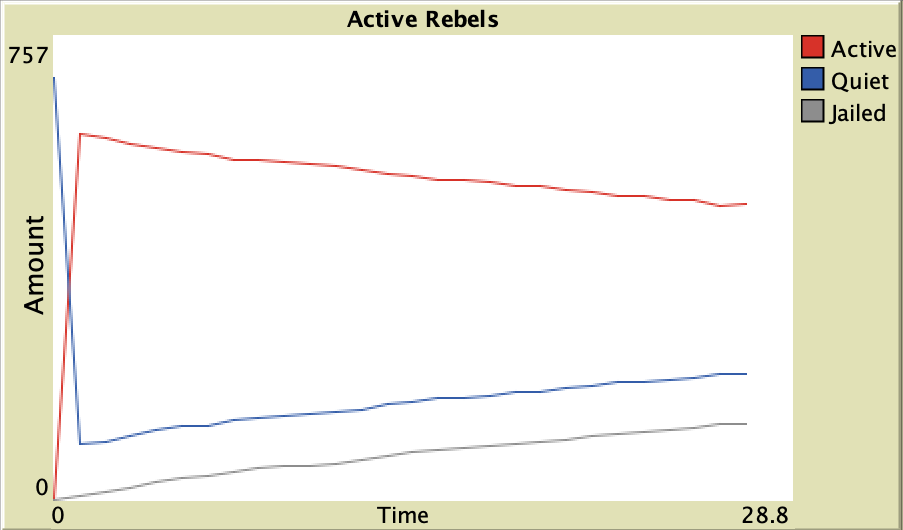
\includegraphics[width=0.9\linewidth, %height=5cm]{BURST_COMM_OFF.png}
%\caption{DISABLED}
%\label{fig:subim3}
%\end{subfigure}
%\begin{subfigure}{0.5\textwidth}
%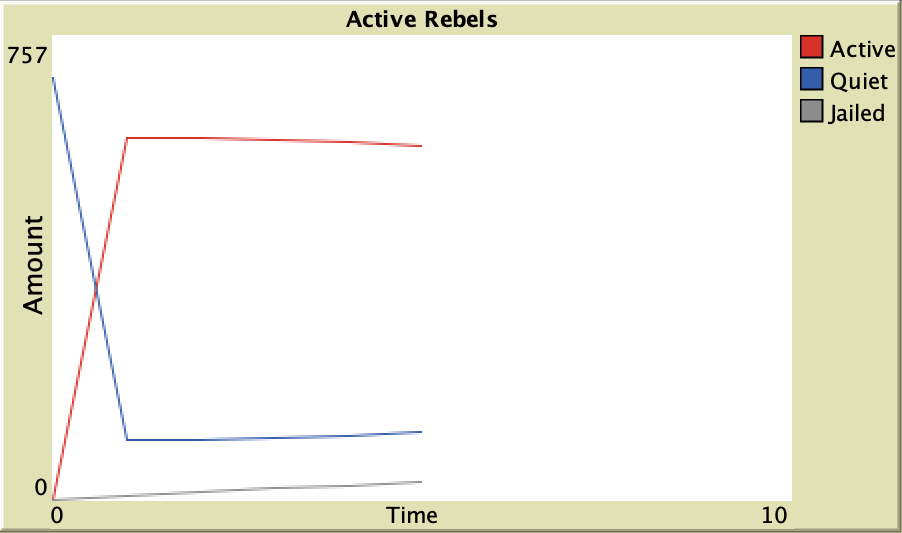
\includegraphics[width=0.9\linewidth, %height=5cm]{BURST_COMM_ON_copy.png}
%\caption{ENABLED}
%\label{fig:subim4}
%\end{subfigure}

%\caption{Communication attribute influencing initial outburst in rebel behaviour}
%\label{fig:fig3}
%\end{figure}

%\textbf{Special case observation – jail term “INFINITY”} - 
%With the least possible “Initial-cop-density” – 0.005, if the attribute is set to infinity for jail term after an initial outburst of active rebels, they are all jailed quickly and the rebellion is nullified in no time. For the same scenario if news was available to the rebels, we see the number of rebels being jailed reduced and the time taken to quell the rebellion takes even longer as the communication \textit{(News ratio = 1.0)} helps the rebels to decide better and keep the movement going longer. We also see the initial burst in rebel behaviour changes considerably when there is communication as shown in Figure \ref{fig:fig3}.
% trial values(Values – IPD: 0.49; ICD: 0.005; Legitimacy: 0.16; AV: 1.0; CV: 1.0; Jail term – infinity; Movement: ON; News ratio: 1.00)



\subsection{Summary of findings with the Beta Model}
The Beta model is implemented on top of Epstein's model \cite{epstein2002modeling} along with few additions/modifications. Firstly, movement of rebels and cops are being done strategically instead of random. Secondly, cop defection is modeled using some attributes for cops. The key findings due to movement would be that current model depicts real world scenario in which each agent takes next step based on best possible outcome instead of moving randomly. This causes clustering, local hot-spot as well as grouping of rebels. In addition wait time between subsequent outburst also reduces and we get realistic value of number of agents in the complex system. For the social media part, the main finding is that an increase in communication between rebels mainly leads to rebels being jailed less, which in turn leads to more active rebels (Figures \ref{fig:avoidanceRun1}, \ref{fig:subimrun2Avoid}, \ref{fig:subimrun2Custom}, \ref{fig:subimrun3Avoid}, \ref{fig:subimrun3Custom}). We expect that the future expansion of the perceived legitimacy will lead to a faster and easier spread of activity in the rebels. The key findings of cop defection model is that if a system has defected cops who support rebellion cause, the active rebels will increase when compared to that of the scenario with ideal cops (no defected cops). This can be observed in Figure \ref{fig:figCopDefection}. With the use of dynamic attributes to model the cop defection in our future work, we expect to see more interesting observations in the rebellion dynamics.


\section{Conclusion}
\subsection{Discussion}
% What do you take away from your project?
% What did you learn?

Agent based models offer intuition for understanding the complex dynamics of civil violence in a rebellion. This helps the policy making stake holders to design effective and efficient policies to anticipate and deal with such rebellions. Epstein's model shows the nuances of how and why a population transitions from being quiet to a state of rebellion\cite{epstein2002modeling}. Especially, the changes that need to happen that can start a rebellion can be seen clearly in the simulation. We observed patterns that are consistent with Epstein's model \cite{epstein2002modeling} from the simulations of our implementation of the model. The observations show us what tipping points cause an aggrieved population to start rebelling and they are as follows:
\begin{itemize}
    \item The rebels can quickly become quiet when cops are in their vicinity, only to become actively rebellious as soon as the cops move away.
    \item Because of the random motion of both rebels and cops, rebellions often happen in quick, local outbursts. The mildly aggrieved rebels become active to join the rebellion in the low cop density zones.
    \item With a small, incremental decrease of legitimacy, the frequency of rebellion does not increase. But, a sudden decrease instantly causes a rebellion to occur.
    \item A small, incremental decrease of the cop density does cause a rebellion at a certain point.
\end{itemize}
Furthermore, we observed the effects of a more coordinated rebel movement. This coordination was the result of social media, where access to social media meant that rebels were able to spread information about the cops' location. When such information is known to the rebels, they are able to keep the rebellion going for longer. In the cop defection model, we observe that the number of active rebels increase when compared to that of the case where cop defection is disabled.

% General summary

\subsection{Relevance}
% Key question 5: What is the relevance of this work?
% Which new questions do you have now?
% Do you results suggest future research directions?

In recent times, we have witnessed large protests, sometimes leading to violent confrontations. Often, it is seen that a centralized entity tries to control a decentralized entity or a centralized group of protesters in general. With advancement in technology Epstein's model is outdated in terms of relevance to actual scenario currently witnessed in protests. %Social media and Cop defection (modelled after varying legitimacy perceptions) play vital roles in the dynamics of the protests. This study on model formulation and implementation for social Media and cop defection lets us know on the extent to which Epstein's model fare in context to current world scenarios. \\  %In the United States of America, protests began in several cities following the results of 2020 presidential election. There were multiple events that led the protests transition to riots with violent confrontations between some protesters and police forces with multiple casualties \cite{enwiki:usprotest}. A few more examples that are worth mentioning are the Hong Kong protests \cite{enwiki:hongkongprotest} and the Indian farmers protests \cite{enwiki:indiafarmprotest} which turned into violent confrontation between some protesters and the police force. In case of the Hong Kong riots, there is also a report of police indulgence in misconduct. This reportedly led to reduced approval rating of the police force \cite{enwiki:hongkongprotest}.

%The protests and rebellions have been a powerful means for civilians to demand and sometimes achieve political change. We have observed protests and rebellious activities throughout history. Some policy makers fear the power of civilians through rebellions \cite{thecrowd}. These fears are amplified in the modern days, with the advent of technology, mobile communication devices, and digital media networks \cite{phdthesisfaris, Rheingold2002SmartMT}. Ubiquitous access to Information and Communication Technologies (ICT) and smartphones dramatically changed the dynamics of social conflict phenomena \cite{phdthesisfaris, twitterarticle}. The importance of understanding and if possible predicting and eventually controlling the protests and rebellions in the number, variety, and intensity cannot be overemphasized\cite{stateofartreview}.
Although Epstein's model has few strengths such as simplicity, the choice of attributes used for modeling rebels' behaviour and its explanatory power. But there are significant setbacks in the model, such as 
\begin{itemize}
    \item the modeling of cops’ behaviour is very crude and does not include scenarios where cops defect and support the rebels or if the cops indulge in misconduct,
    \item cumulative (memory) effects from previous events do not change either the agents’ state or the simulation attributes and
    \item the model attributes do not take into account the current social context.
\end{itemize}
We are looking at the key attributes that has major impact in the current scenarios while modeling the system to build a new perspective, and anticipate possible research trends in this area. We have taken into account the scenarios of cops' defection using dynamic attributes of the rebellion dynamics and the effects of digital media in the rebellion dynamics as an extension of Epstein's model. With these approaches, we expect to achieve better understanding of protests and rebellion dynamics in the recent times.

\subsection{Team Work}
% How did you work together as a team?
% Who contributed how to this report and to the implementation?
% What should you have done differently?

There is an active participation and co-operation from all the team members towards the project. The contributions to the report is as follows
\begin{itemize}
    \item Modified model for Cop Defection - Abhishek Ramanathapura Satyanarayana
    \item Further Mathematical modelling of Cop defection - Sam Reswinraj Abraham
    \item Modified model for social media  - Niels Burgler \& Amit Bharti
    \item Implementation of models in Netlogo, Alpha version infusion with Beta version, Conclusion, Relevance and References - Everyone
\end{itemize}

%The contributions to our model implementation is currently by Niels Burgler since the rest of us are still learning Netlogo. The code review is done by everyone. The team members who are new to Netlogo should have researched more on hands-on Netlogo but everyone is learning. The implementation will include active contributions from the other members for the beta and the final versions.

% This will print you references, please do not change it.
\printbibliography

\end{document}